\chapter{Diseño e implementación} % Main chapter title

\label{Chapter3} % Change X to a consecutive number; for referencing this chapter elsewhere, use \ref{ChapterX}

\definecolor{mygreen}{rgb}{0,0.6,0}
\definecolor{mygray}{rgb}{0.5,0.5,0.5}
\definecolor{mymauve}{rgb}{0.58,0,0.82}

%%%%%%%%%%%%%%%%%%%%%%%%%%%%%%%%%%%%%%%%%%%%%%%%%%%%%%%%%%%%%%%%%%%%%%%%%%%%%
% parámetros para configurar el formato del código en los entornos lstlisting
%%%%%%%%%%%%%%%%%%%%%%%%%%%%%%%%%%%%%%%%%%%%%%%%%%%%%%%%%%%%%%%%%%%%%%%%%%%%%
\lstset{ %
  backgroundcolor=\color{white},   % choose the background color; you must add \usepackage{color} or \usepackage{xcolor}
  basicstyle=\footnotesize,        % the size of the fonts that are used for the code
  breakatwhitespace=false,         % sets if automatic breaks should only happen at whitespace
  breaklines=true,                 % sets automatic line breaking
  captionpos=b,                    % sets the caption-position to bottom
  commentstyle=\color{mygreen},    % comment style
  deletekeywords={...},            % if you want to delete keywords from the given language
  %escapeinside={\%*}{*)},         % if you want to add LaTeX within your code
  %extendedchars=true,             % lets you use non-ASCII characters; for 8-bits encodings only, does not work with UTF-8
  %frame=single,	                 % adds a frame around the code
  keepspaces=true,                 % keeps spaces in text, useful for keeping indentation of code (possibly needs columns=flexible)
  keywordstyle=\color{blue},       % keyword style
  language=[ANSI]C,                % the language of the code
  %otherkeywords={*,...},          % if you want to add more keywords to the set
  numbers=left,                    % where to put the line-numbers; possible values are (none, left, right)
  numbersep=5pt,                   % how far the line-numbers are from the code
  numberstyle=\tiny\color{mygray}, % the style that is used for the line-numbers
  rulecolor=\color{black},         % if not set, the frame-color may be changed on line-breaks within not-black text (e.g. comments (green here))
  showspaces=false,                % show spaces everywhere adding particular underscores; it overrides 'showstringspaces'
  showstringspaces=false,          % underline spaces within strings only
  showtabs=false,                  % show tabs within strings adding particular underscores
  stepnumber=1,                    % the step between two line-numbers. If it's 1, each line will be numbered
  stringstyle=\color{mymauve},     % string literal style
  tabsize=2,	                     % sets default tabsize to 2 spaces
  title=\lstname,                  % show the filename of files included with \lstinputlisting; also try caption instead of title
  morecomment=[s]{/*}{*/}
}


%----------------------------------------------------------------------------------------

Este capítulo describe el diseño y la implementación de cada uno de los componentes que conforman el sistema.
Se explican las decisiones de diseño, los flujos de trabajo y los aspectos técnicos involucrados en la construcción de cada módulo principal.

%---------------------------------------------------------------------------------------
\section{Arquitectura del sistema}

El sistema está diseñado para permitir la implementación y operación de un chatbot mediante un enfoque de recuperación aumentada por generación. 
Se implementó una arquitectura modular, basada en servicios en la nube, que facilita la escalabilidad y el mantenimiento del chatbot, y permite 
una actualización ágil de los componentes y una experiencia optimizada para los usuarios finales. En la figura \ref{fig:architecture} se ilustra
el diagrama de arquitectura, donde se observan la totalidad de los componentes que conforman el sistema.

En primer lugar, los usuarios interactúan con el chatbot a través de una interfaz gráfica (desarrollada con NextUI y deployada en Azure Static Web App), 
donde consultan por la información deseada. Estas consultas son luego transferidas al servidor (Azure App Service) a través de una API desarrollada 
con la librería FastAPI. Una vez allí, se realiza un proceso de búsqueda por similitud que toma la consulta del usuario y la compara con la información
disponible en la base de datos (Azure AI Search), con el objetivo de identificar aquellos fragmentos más relevantes. Previamente, un administrador
debe haber cargado aquellos documentos que conforman la base de conocimiento del chatbot en un repositorio de GitHub, tras lo cual se ejecuta la 
automatización que procesa los documentos y los envía a la base de datos.

Para alimentar esta base de conocimiento, un administrador carga los documentos en un repositorio de GitHub, donde una automatización (desarrollada 
utilizando GitHub Actions) procesa los documentos y los transfiere a la base de datos.

Finalmente, la consulta del usuario y los fragmentos relevantes se envían al modelo LLM (desplegado en el servicio Azure OpenAI), que genera una 
respuesta contextualizada. Esta respuesta es devuelta a la interfaz gráfica para ser presentada al usuario.

Además, se incluye una pequeña base de datos adicional (Azure Table Storage) que se utiliza para guardar el \textit{feedback} de los usuarios, 
para así obtener métricas del desempeño del chatbot.  

\vspace{10mm}

\begin{figure}[ht]
	\centering
	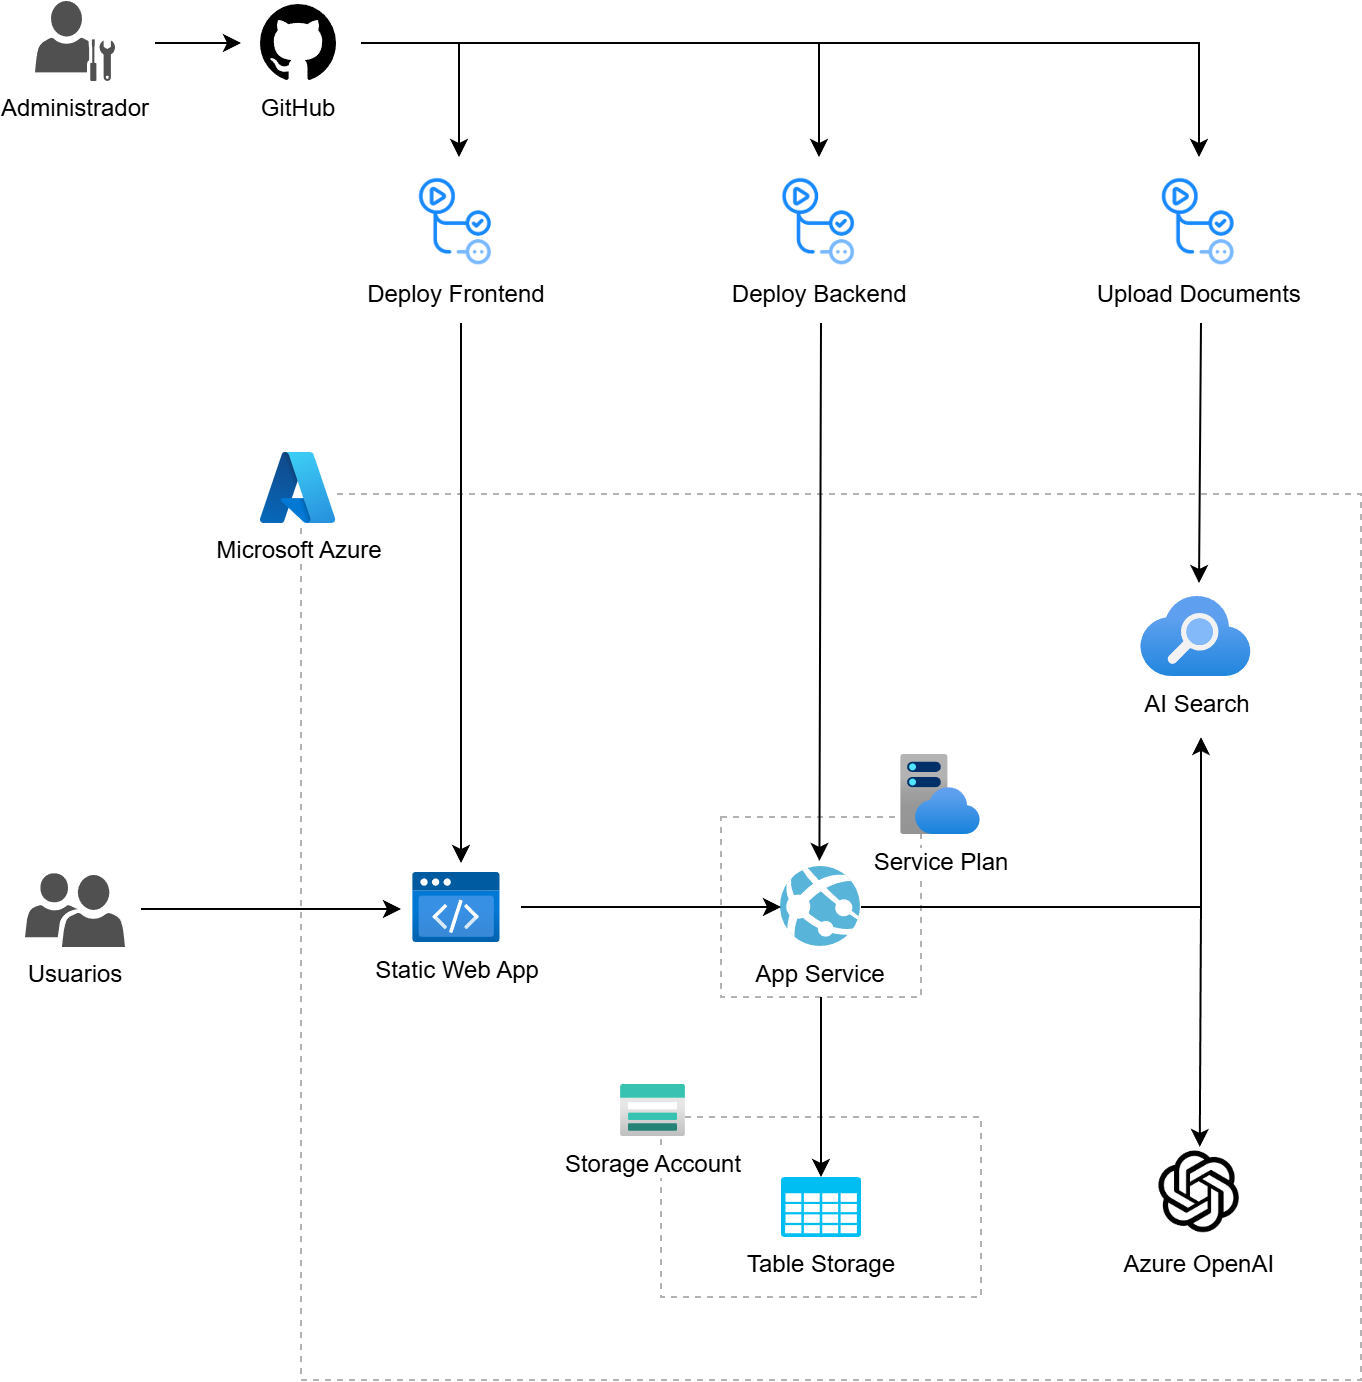
\includegraphics[scale=.55]{./Figures/arquitectura.png}
	\caption{Diagrama de la arquitectura del sistema.}
	\label{fig:architecture}
\end{figure}

\vspace{5mm}

%---------------------------------------------------------------------------------------
\section{Configuración de la infraestructura en la nube}

Para garantizar el despliegue, disponibilidad y escalabilidad del sistema, se configuró una infraestructura en la nube basada en Microsoft Azure. 
A continuación, se describen los pasos principales para la configuración de cada recurso empleado en el proyecto.

\subsection{OpenAI Service}

El servicio de Azure OpenAI proporciona acceso a los potentes modelos de lenguaje de OpenAI, incluidos los modelos más recientes. 
Estos modelos pueden adaptarse fácilmente a tareas específicas, como en nuestro caso es la generación de contenido.

En la tabla \ref{tab:config-openai} se presenta un resumen de las configuraciones realizadas. 
Se seleccionó \textit{East US} como región, junto con el modelo de precios \textit{Standard S0}, 
adecuado para balancear el costo y el rendimiento del sistema.

Como medida de seguridad, se configuraron reglas de red para restringir el acceso únicamente al rango 
de direcciones IP del \textit{backend} alojado en Azure App Service. Esto asegura que solo las solicitudes provenientes de la 
aplicación puedan acceder al modelo de lenguaje, lo que protege el servicio de accesos no autorizados.

Una vez desplegado el recurso, fue necesario seleccionar y desplegar los modelos específicos requeridos para la funcionalidad del chatbot. 
En este caso, se optó por los siguientes modelos:

\begin{itemize}
	\item \textit{GPT-4o} como modelo de lenguaje para generación de respuestas. Este modelo está diseñado para brindar velocidad 
  y eficiencia, iguala la inteligencia de su antecesor \textit{GPT-4 Turbo}, y es notablemente más eficiente al entregar texto al 
  doble de velocidad y a la mitad del costo. Además, exhibe el rendimiento más alto en idiomas distintos del inglés en comparación 
  con los modelos de OpenAI anteriores.
	\item \textit{Ada-002} para el cálculo de \textit{embeddings} de texto. Este modelo supera a todos los modelos de \textit{embeddings} 
  anteriores en tareas de búsqueda de texto y similitud de oraciones.
\end{itemize}

Adicionalmente, es fundamental obtener el \textit{endpoint} y la \textit{key} del servicio, valores que se utilizan luego para la comunicación programática 
con Azure OpenAI. Estos datos se almacenan en el \textit{backend} como variables de entorno para que el sistema pueda acceder al servicio de manera segura.

\begin{table}[h]
	\centering
	\caption[Configuración de Azure OpenAI]{Configuración de Azure OpenAI}
	\begin{tabular}{l c}    
		\toprule
		\textbf{Configuración} 	 & \textbf{Detalles} 	\\
		\midrule
		Región &	East US 				\\		
		Nivel de precios & Standard S0				\\
		Reglas de Firewall & Rango IP de App Service 				    \\
    Modelos desplegados	& gpt-4o				\\
            	 & text-embeddings-ada-002			    \\
    Credenciales	& Endpoint y Key 		    \\
		\bottomrule
		\hline
	\end{tabular}
	\label{tab:config-openai}
\end{table}

\subsection{AI Search}

\subsection{App Service }

\subsection{Static Web App}

\subsection{Table Storage}

%---------------------------------------------------------------------------------------
\section{Procesamiento de los documentos}

%---------------------------------------------------------------------------------------
\section{Lógica de comunicación entre el usuario y el modelo}

%---------------------------------------------------------------------------------------
\section{API}

%---------------------------------------------------------------------------------------
\section{Interfaz de usuario}

%---------------------------------------------------------------------------------------
\section{Pipelines de despliegue automático}